\documentclass[12pt,letterpaper,english,bibliography=totocnumbered, abstract=on]{scrartcl}

\usepackage{indentfirst}
\usepackage[titletoc]{appendix}
\usepackage{fullpage}
%\usepackage{subfiles}
\usepackage[T1]{fontenc}
\usepackage[latin9]{inputenc}
\usepackage{color}
\usepackage{babel}
\usepackage{verbatim}
\usepackage[unicode=true,pdfusetitle,
bookmarks=true,bookmarksnumbered=false,bookmarksopen=false,
breaklinks=true,pdfborder={0 0 0},pdfborderstyle={},backref=false,colorlinks=true]
{hyperref}
\hypersetup{linkcolor=blue,citecolor=blue,urlcolor=blue}

\usepackage{booktabs}
\usepackage{multirow}
\usepackage{adjustbox}
\usepackage{threeparttable}
\usepackage[table]{xcolor}
\usepackage{csquotes}
\usepackage{soul} % for hiliting text: \hl

\usepackage[backend=biber, style=authoryear, maxbibnames=99, dashed=false]{biblatex}
\setlength\bibitemsep{2\itemsep}
%\addbibresource{mylibrary.bib}
%\addbibresource{CRB.bib}

\usepackage{pdfpages}
\usepackage{float} % Allows use of H to place floats

\usepackage{pgfgantt}

\usepackage{framed}

% Prevent page breaks within paragraphs
% https://tex.stackexchange.com/questions/21983/how-to-avoid-page-breaks-inside-paragraphs
\widowpenalties 1 10000

\begin{document}

\titlehead{Technical Report}

\title{\textit{Aulacaspis yasumatsui} on \textit{Cycas micronesica} Growing Outside the Conservation Plots on Tinian}

\author{Aubrey Moore}

\date{March 23, 2022\\Revised March 24, 2022}

\maketitle
%\footnote{\url{https://github.com/aubreymoore/2020-FS-CRB-biocontrol-project/blob/master/combined-proposal.pdf}}
\newpage
\tableofcontents

\pagebreak

The most recent version of this document may be downloaded from \url{https://github.com/aubreymoore/Tinian-cycad-images/raw/main/report/tinian_cycad_images.pdf}.

All data and code used in this report are available in a public GitHub repository at
\url{https://github.com/aubreymoore/Tinian-cycad-images}.

\section{Introduction}

Ken Puliafico very kindly shared 81 high quality close-up images of \textit{Cycas micronesica} growing on Tinian outside the conservation plots. These were recorded using a Google Pixel 3a cell phone. Some of the images clearly indicated CAS infestation. Images were used to generate an interactive web map to facilitate visualization. 

\begin{figure}[h]
	\centering
	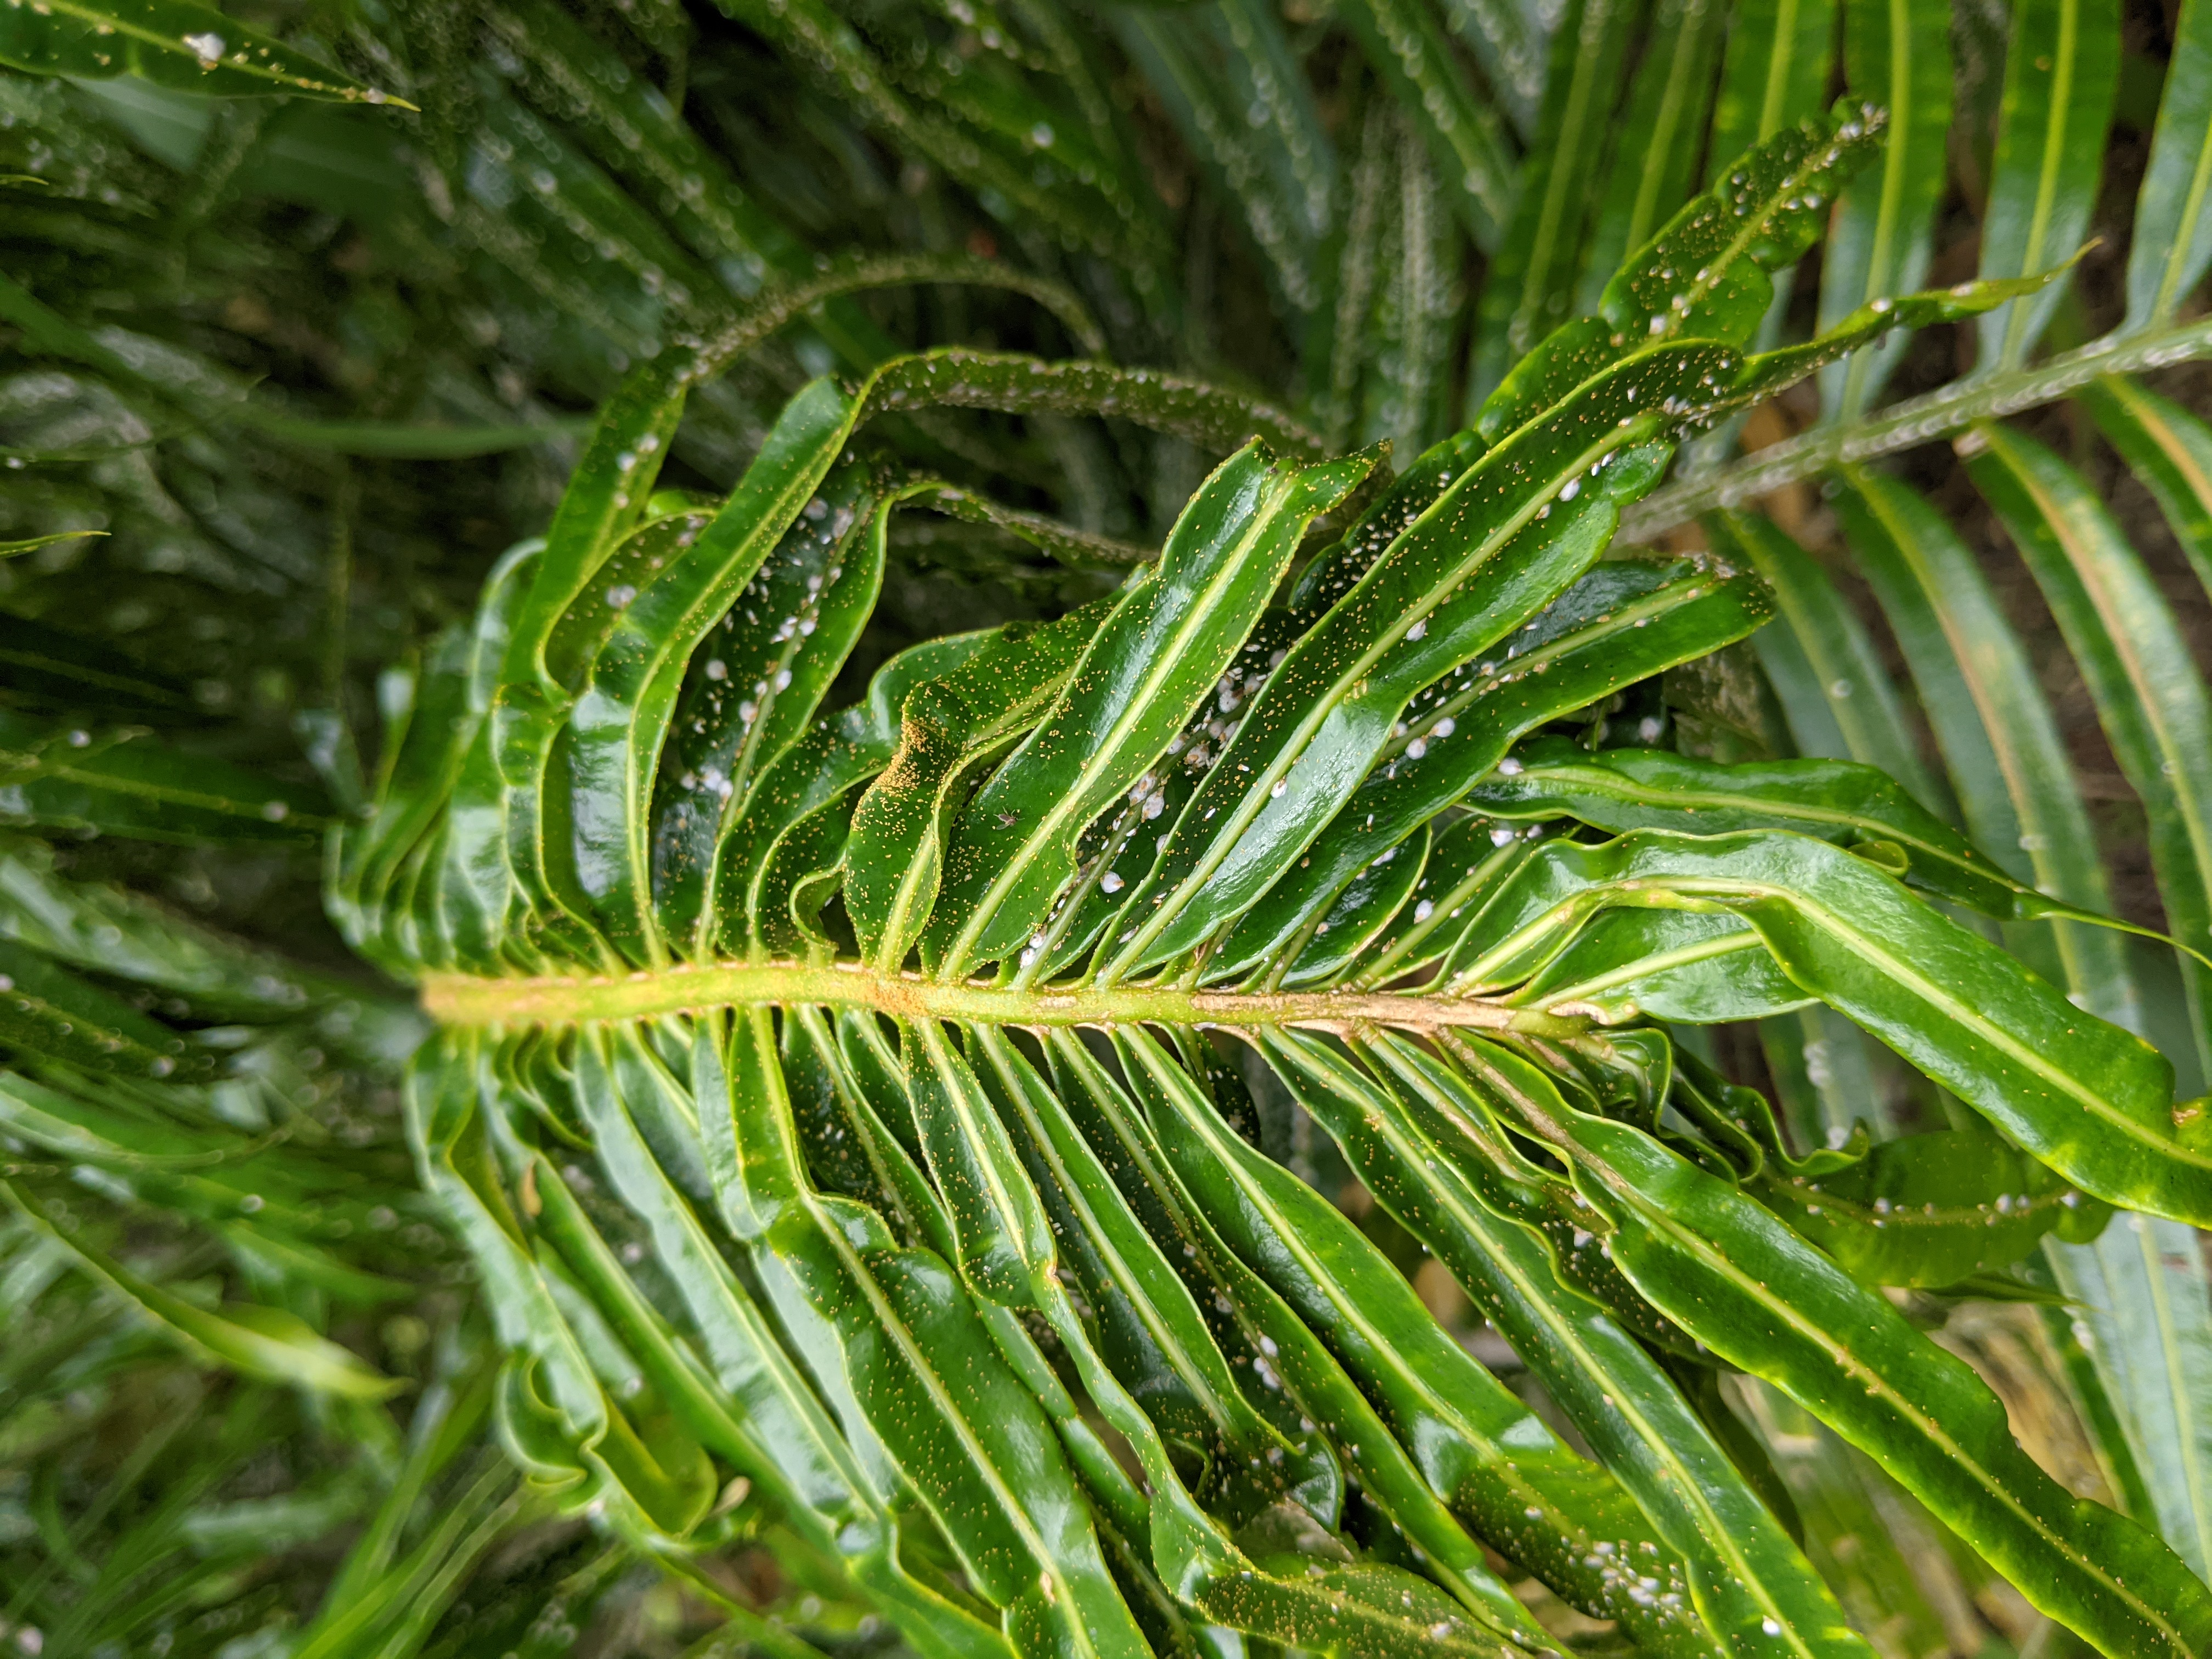
\includegraphics[width=1\linewidth]{../images/PXL_20210725_040405506}
	\caption{This image of \textit{Cycas micronsesica} leaflets infested with CAS was taken by Ken Puliafico on Mount Lasu, Tinian on July 25 2021. It is remarkable because large numbers of scale crawlers are clearly visible.}
	\label{fig:crawlers}
\end{figure}

\section{Methods}

All data processing was performed using free, open-source software.

Data were prepared using Python 3 in a \href{https://github.com/aubreymoore/Tinian-cycad-images/blob/main/code/select\_1\_image\_at\_each\_location.ipynb}{Jupyter Notebook} which performed the following steps.

\begin{itemize}
	\item Latitude, longitude and time stamp were extracted from each image file. \item Multiple images taken at each unique location. A folder was created for each unique location and it was populated with images from that location.
	\item All images in the above folders were examined for presence of cycad aulacaspis scale and an examplar image for the location was selected. This step was performed manually.
	\item Data for each unique location were stored in a \href{https://github.com/aubreymoore/Tinian-cycad-images/blob/main/images.csv}{CSV file} which was subsequently used for generating a web map.
\end{itemize}

An interactive web map was prepared using QGIS 3.22. The QGIS project file is available in the GitHub repository.

\clearpage
\section{Results}

\begin{figure}[h]
	\centering
	\includegraphics[width=1\linewidth]{"Screenshot from 2022-03-24 09-21-42"}
	\caption{Map showing 3 clusters of \textit{Cycas micronesica} plants. Images plants in the most southern cluster indicate CAS infestation.}
	\label{fig:screenshot-from-2022-03-24-09-21-42}
\end{figure}

\begin{figure}[h]
	\centering
	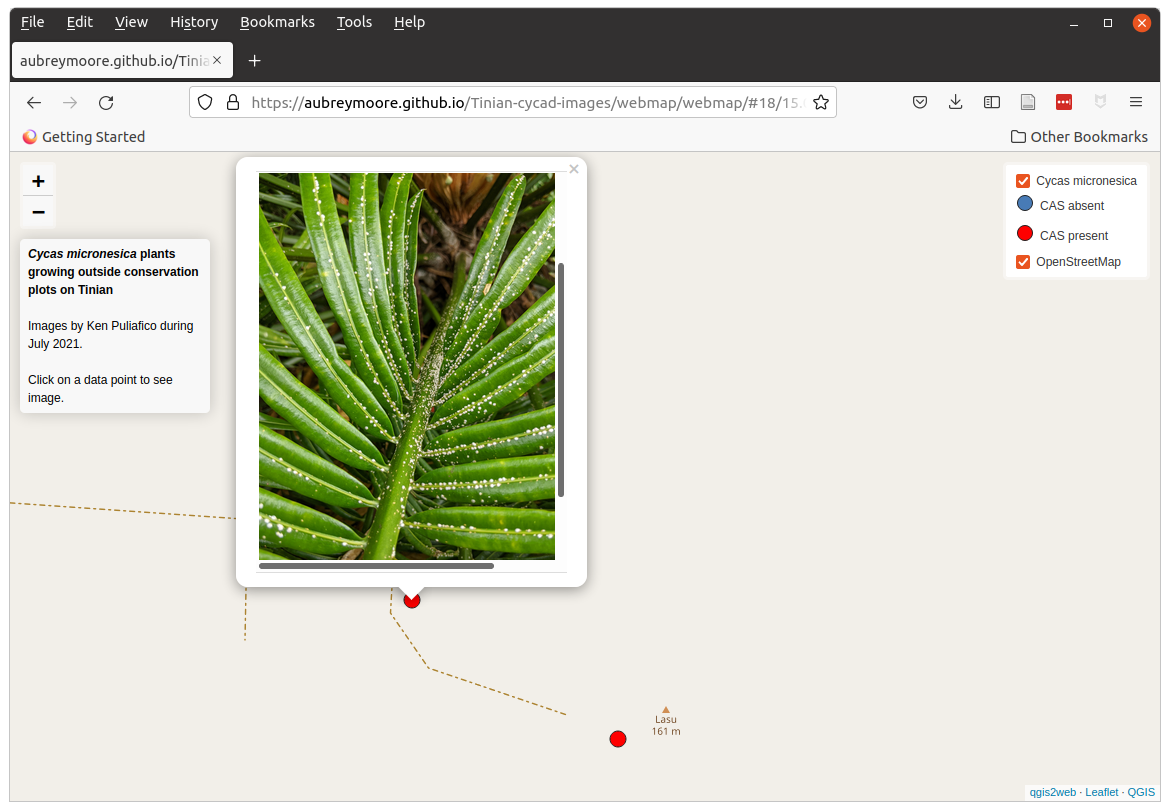
\includegraphics[width=1\linewidth]{webmap}
	\caption{Interactive web map of \textit{Cycas micronesica} locations and images.
	Publicly available at \url{https://aubreymoore.github.io/Tinian-cycad-images/webmap/webmap/}}
	\label{fig:webmap}
\end{figure}

\end{document}
